\documentclass[ignorenonframetext,hyperref={pdftex,unicode}]{beamer}
%\documentclass[aspectratio=169,ignorenonframetext,hyperref={pdftex,unicode}]{beamer}  %соотношение 16:9

\newcommand{\shellcmd}[1]{
\indent\texttt{\footnotesize\# #1}
}
\newcommand{\cfgline}[1]{
\indent\texttt{\footnotesize #1}
}

\usepackage{amssymb,amsmath,mathtext} %поддержка формул и русского текста в них
\usepackage{indentfirst,amsfonts} %поддержка русского стиля оформления текста и формул
%\usepackage{makecell,multirow,longtable} %поддержка таблиц занимающих несколько страниц

\usepackage[english,russian]{babel}
\usepackage[T2A]{fontenc}
\usepackage[utf8]{inputenc} %кодировка исходника

% for hyperlinks
\usepackage{hyperref}
% for strike-out text
\usepackage[normalem]{ulem}

\ifpdf
        \usepackage{cmap} % чтобы работал поиск по PDF
        %\usepackage[pdftex]{graphicx}
        \pdfcompresslevel=9 % сжимать PDF
\else
        \usepackage{graphicx}
\fi

\usetheme{Samsolutions} %корпоративная тема

%\setbeamercovered{transparent} %полупрозрачные скрытые элементы

\title{Hack the Hackpad} %название презентации
\subtitle{Першая спроба публічнага кіравання задачамі для лінуксовак} %подназвание
\author["Андрэй Захарэвіч"]{Андрэй Захарэвіч\\ andrej@zahar.ws} %автор


\begin{document} %начало документа

\frame{\titlepage} % Создание заглавной страницы


\section{Што рабілі і навошта} %названия секций для оглавления

\begin{frame}{З чаго пачыналася} %новый слайд и его название
	Што хацелі атрымаць:
	\begin{itemize}
		\item Публічна даступны спіс задач да лінуксовак\pause
		\item Магчымасць дадаваць новыя задачы\pause
		\item Магчымасць браць на сябе існуючыя задачы 
	\end{itemize}
	\begin{center}
 		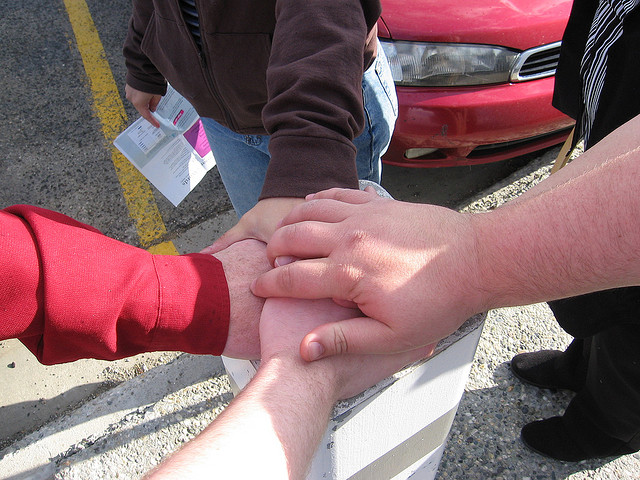
\includegraphics[height=0.5\textheight,keepaspectratio]{145149313_c9c75df6f8_z} %так вставляется картинка
	\end{center}
\end{frame} %конец слайда

\section{Hackpad}
\begin{frame}{Новы цудоўны свет}
	Пасля абмеркаванняў на лінуксоўцы і першых спроб паглядзець на інструменты пачалі эксперыментаваць з \href{https://hackpad.com/}{Hackpad}. І мне гэта нават вельмі падабалася некаторы час. 
	\begin{center}
		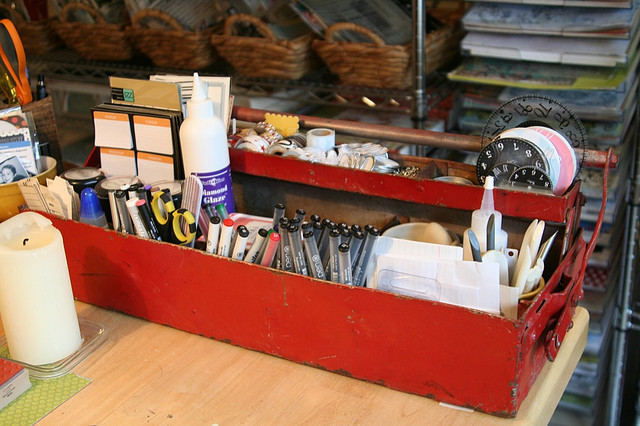
\includegraphics[height=0.5\textheight,keepaspectratio]{502240730_b00feb15b0_z}
	\end{center}
\end{frame}

\subsection{Перавагі}
\begin{frame}{Перавагі і выгоды}
	Што было добра:
	\begin{itemize}
		\item Спіс даступны без аніякай аўтарызацыі\pause
		\item Лёгка дадаць новыя задачы, ці пазначыць сябе (у каменце) адказным за існуючыя\pause
		\item Лёгка пазначыць задачу выкананай
	\end{itemize}
	\begin{center}
		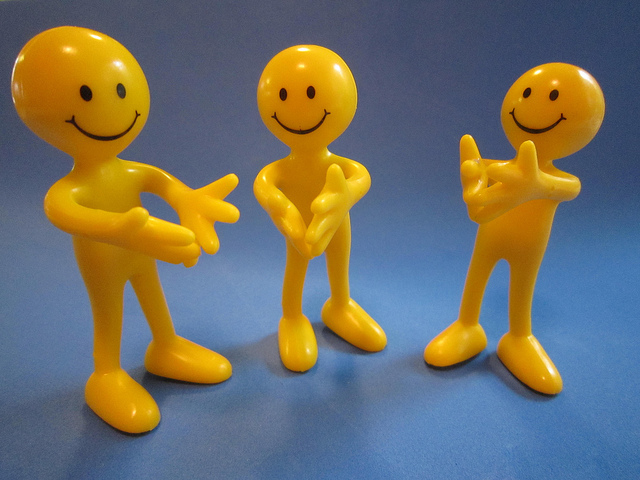
\includegraphics[height=0.5\textheight,keepaspectratio]{5129669316_a14566600e_z}
	\end{center}
\end{frame}

\subsection{Недахоп}
\begin{frame}{Першы сабака бліну}
	Але літэральна ў першыя ж гадзіны высветліўся дробны недахоп, які псаваў усё:
	\begin{center}
		 \textsc{Яно не заўсёды запамінае расстаўленыя птушачкі выкананых задач!}
	\end{center}
	І гэты касяк усплываў увесь час і не толькі ў мяне.
\end{frame}

\subsection{Зварот у тэхпадтрымку}
\begin{frame}{Звярніцеся за падтрымкай}
	Я, натуральна ж, напісаў ліст ў тэхпадтрымку. І, нават, пастараўся не ўжываць англійскіх словаў з чатырох літар.
	\begin{center}
 		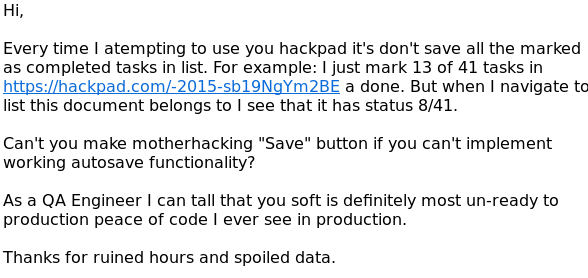
\includegraphics[height=0.5\textheight,keepaspectratio]{support0}
	\end{center}
\end{frame}

\begin{frame}{Не кажы куды я мушу ісці…}
	І яны мне нават адказалі. Дарэчы, таксама не ўжывалі словаў з чатырох літар. Але ўсё ж параілі мне паісці некуды…
	\begin{center}
 		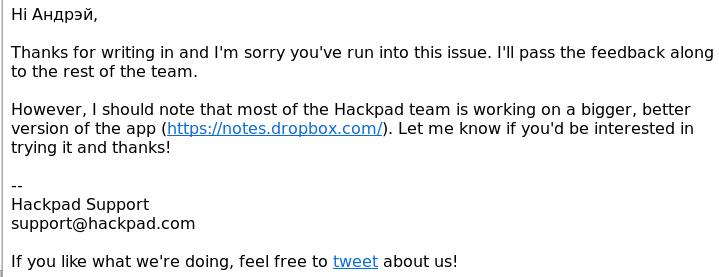
\includegraphics[height=0.3\textheight,keepaspectratio]{support1}
	\end{center}
\end{frame}

\section{Што рабіць далей?}
\begin{frame}{Што рабіць далей?}
	Мне здаецца, што далей мы можам:
	\begin{itemize}
		\item Карыстацца далей, пазначаючы выкананыя задачы, напрыклад з дапамогай [*]\pause
		\item Пераключыцца на \href{http://kanboard.net/}{kanboard}\pause
		\item Пераключыцца на нешта больш вялікае і цяжкае (\href{http://www.redmine.org/}{Redmine}, \href{http://trac.edgewall.org/}{trac})
	\end{itemize}
	\begin{center}
 		
\includegraphics[height=0.5\textheight,keepaspectratio]{Pn-slogan-zakon}
	\end{center}
\end{frame}

\frame{\finalslide{Пытанні ці прапановы?}} %слайд вопросы?

\begin{frame}{Ужытыя малюнкі}
	\begin{thebibliography}{10}
	\beamertemplatetextbibitems
	\bibitem{}
		{\sc \href{https://www.flickr.com/photos/fncll/145149313}{Collaboration}} by {\sc \href{https://www.flickr.com/photos/fncll/}{Chris Lott}};
	\bibitem{}
		{\sc \href{https://www.flickr.com/photos/aliedwards/502240730}{red tool box}} by {\sc \href{https://www.flickr.com/photos/aliedwards/}{Ali Edwards}};
	\bibitem{}
		{\sc \href{https://www.flickr.com/photos/katerha/5129669316}{If you're happy and you know it, Clap your hands}} by {\sc \href{https://www.flickr.com/photos/katerha/}{Kate Ter Haar}};
	\bibitem{}
		{\sc \href{https://en.wikipedia.org/wiki/Five-year\_plans\_for\_the\_national\_economy\_of\_the\_Soviet\_Union\#/media/File:Pn-slogan-zakon.jpg}{Лозунг «План — закон, выполнение — долг, перевыполнение — честь!» в здании Ольховско-Батьковского торфяного предприятия в Кубринске, Переславский район.}} by {\sc \href{https://commons.wikimedia.org/wiki/User:\%D0\%9F\%D0\%B5\%D1\%80\%D0\%B5\%D1\%81\%D0\%BB\%D0\%B0\%D0\%B2\%D1\%81\%D0\%BA\%D0\%B0\%D1\%8F\_\%D0\%BD\%D0\%B5\%D0\%B4\%D0\%B5\%D0\%BB\%D1\%8F}{Газета «Переславская неделя» / Ю. Н. Частов /}}.
	\end{thebibliography}
%"Pn-slogan-zakon" by Газета «Переславская неделя» / Ю. Н. Частов / CC-BY-SA 3.0. Licensed under CC BY-SA 3.0 via Commons - https://commons.wikimedia.org/wiki/File:Pn-slogan-zakon.jpg#/media/File:Pn-slogan-zakon.jpg	
\end{frame}

\end{document}
